\section{Cryptographic Engine}\label{arch:crypto}

The design of the TEM's cryptographic engine has a huge impact on the TEM's
adoption rate. Cryptography algorithms account for most of the cost, die
size, and power consumption of a secure chip. Some cryptographic methods
carry legal implications, so the choices made here can place restrictions on
the TEM's adoption.

Furtermore, some algorithms incur a large computational effort, so incorporating
them has a severe impact on an application's response time. For example,
generating a 2048-bit RSA key takes a non-trivial amount of time, even on the
most powerful desktops available today. In order to alleviate this issue, the
functionality of the cryptographic engine is usually implemented in
hardware\footnote{Most chip vendors call it a cryptographic accelerator.}.

Fortunately, the Trusted Computing Group has already found good answers to
all of the concerns mentioned above, in their design of the Trusted Platform
Module (TPM) \cite{tcpa2007}. Therefore, the TEM's cryptographic engine
architecture builds heavily on the design of its counterpart in the TPM. This
section discusses the resulting design, and explains the significance of its
elements, in the context of the TEM.

\subsection{Random Number Generator}\label{arch:crypto_rng}
Genuine random numbers are needed as material for key generation, and to
implement nonces, which can be used to build freshness guarantees. Most secure
chips provide a true (hardware-based) random number generator, so this
requirement does not pose implementation issues.

\subsection{Cryptographic Hashes}\label{arch:crypto_hash}
The TEM's cryptographic engine must supply a cryptographically-strong hash.
The TEM needs this ability to verify the integrity of the information in
a bound SECpack, before executing the respective closure. Assuming the binding
process in section \ref{concepts:secpack_binding}, the cryptographic engine is
used to compute $h(\mathcal S || \mathcal P)$, so that it can be
compared with $\mathcal H$.

In order to meet or exceed the security guarantees provided by the TPM, the
cryptographic hash should be at least as strong as SHA1 \cite{eastlake2001rus}.
Fortunately, cryptography research has yielded good hash functions which are
in the public domain.

The TEM does not provide platform attestation to its host computer, so it does
not need to expose cryptographic hashing services directly.

\subsection{Asymmetric Key Cryptography}\label{arch:crypto_asymmetric}
Public key cryptography is the most heavyweight TEM component. It is necessary
because trusted execution requires a shared secret between the TEM and the
party that needs trusted execution guarantees, and secret distribution makes
symmetric encryption impractical.

Fortunately, the cryptographic accelerators on most secure chips provide
the basic asymmetric key operations, namely encryption, decryption, signing,
and signature verification. Also, the most common public encryption scheme,
RSA \cite{rivest1978mod}, has entered the public domain as of year 2000
\cite{rsasec2000}.

In order to be a secure alternative to the TPM, the TEM should support a
public-key encryption algorithm that yields at least the same security as
2048-bit RSA.

\subsubsection{Asymmetric Key Generation}
The only operation posing challenges is asymmetric key generation. In RSA, key
generation demands more resources than the other operations, by an order of
magnitude.

Key generation is not a hard requirement for a TEM. A manufacturer can choose
to generate the TEM's Private Endorsement Key outside the chip, at manufacturing
time, and then embed the key inside the TEM. The chain of trust in section
\ref{concepts:trust_chain} remains valid, as long as the manufacturer erases a
TEM's Private Endorsement Key from any medium outside that TEM, before the
TEM's Endorsement Certificate is generated.

If a TEM's cryptographic engine is incapable of asymmetric key
generation, TEM anonymity requires extra consideration. The process described
in \ref{concepts:anonymous_trust} can be modified to have the manufacturer's
server generate a User Key for the TEM. The manufacturer's server would then
give Mii the Private User Key (PrivUK) encrypted with the TEM's Public
Endorsement Key (PubEK).

There are secure chips capable of generating 2048-bit RSA keys, and they are
commercially available at reasonably low prices. Therefore, the rest of this
work will assume that the TEM's cryptographic engine provides asymmetric key
generation. It is straightforward to derive the architecture of a TEM without
such a generator, by removing the irrelevant features from the design presented
here.

\subsection{Symmetric Key Cryptography}\label{arch:symmetric_crypto}
Encryption algorithms that use private keys are a couple of orders of
magnitude faster than their public-key counterparts. This makes the
ability of performing symmetric encryption highly desirable.

However, symmetric key cryptography is heavily regulated by most legal systems.
For instance, the DES algorithm \cite{coppersmith1994} is still governed by
export restriction laws in the United States, at the time of this writing.
Furthermore, symmetric encryption is outlawed completetly in some countries. 

Making symmetric key cryptography a part of the TEM architecture would make the
platform vulnerable to legal issues, which would greatly hurt adoption. On the
other hand, private-key encryption cannot be ignored completely, due to the
performance advantages it provides. Therefore, the only logical step is to make
symmetric encryption an optional component of a TEM's cryptographic engine.

If a TEM chooses to offer symmetric encryption, the algorithm should provide at
least the same security guarantees as 128-bit AES \cite{daemen1999apr}. This is
necessary so that symmetric encryption does not become the weakest link in the
system. In other words, secrets protected by symmetric encryption should not be
easier to obtain than secrets protected by other means available in the TEM.

Symmetric cryptography is an optimization, and its presence or absence does
not significantly impact the overall TEM architecture.

\subsection{Secure Key Store}\label{arch:key_store}
A TEM cryptographic engine must provide secure key storage, and this
functionality is provided by the (again, intuitively named) key store. Figure
\ref{fig:key_store} provides a visual summary of the TEM's key store described
in this section.

\begin{figure}[hbtp]
	\center{
		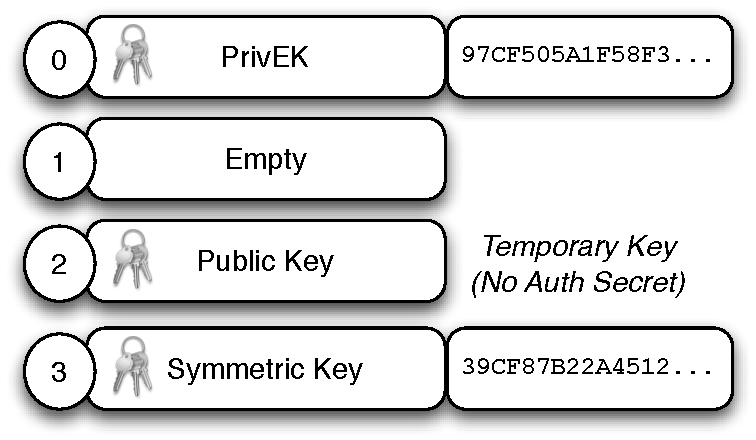
\includegraphics{omnifigs/key_store}
	}
	\caption{Snapshot of a TEM's Key Store}
	\label{fig:key_store}
\end{figure}

The key store is an array of key slots. A slot can store one of the following
encryption keys:
\begin{enumerate}
  \item the public component of an asymmetric key (also called a public key),
  \item the private component of an asymmetric key (also called a private key),
  or
  \item a symmetric key.
\end{enumerate}

The independent treatment of the two components of an asymmetric key is
insipired by the \texttt{javacardx.crypto} API in the JavaCard specification.
The advantage of this is that each key (corresponding to a slot) has
well-defined \texttt{encrypt} and \texttt{decrypt} methods, which would not be
true if both components of an asymmetric key would be amassed together in a
single slot.

A key created during SEClosure execution is temporary, which means it is released
when the closure which created it ends executing. A temporary key becomes
persistent when it is associated with an authorization secret. Authorization
secrets have the same size as a cryptographic hash (section
\ref{arch:crypto_hash}), and are used to regulate access to a TEM's persistent
keys. A closure is allowed to access a persistent key after presenting the
associated authorization secret.

An attractive aspect of this design is that no distinction needs to be made
for storing the TEM's Private Endorsement Key (PrivEK). PrivEK occupies the
first slot in a TEM's key store, and is associated with an authorization value
known only by the platform manufacturer. Furthermore, the manufacturer can
build ``privileged'' SEClosures, which use a TEM's PrivEK to offer additional
functionality. For example, TPM emulation, as well as the TEM anonymizing
scheme in section \ref{concepts:anonymous_trust} can be implemented as a
collection of ``privileged'' SEClosures.

\subsubsection{Considerations for Deleting Keys from the Store}
Allowing unauthorized key deletion does not compromise confidentiality, as no
information is disclosed. However, misuse of key deletion can lead to denial
of service attacks from misbehaving closures.

In order to prevent denial of service, a SEClosure is only allowed to delete from the key store the keys that it would be authorized to use as encryption / decryption keys.

On the other hand, a TEM owner must be allowed to delete persistent keys
from the store without having to know the authorization secret. Otherwise,
misbehaving closures may deny service to the TEM by filling up the key store.

\subsubsection{Motivation for the Key Store}
At a minimum, the cryptographic engine must be able to store the TEM's
Private Endorsement Key (section \ref{concepts:trust_chain}) for the TEM's
life. The engine must also be able to store one additional key, for the
duration of a closure's execution.

However, today's secure chips have enough resources to store many keys
simultaneously. This ability can be leveraged to reduce the number of times
that an often-used key must be loaded into the cryptographic engine. The
optimization can yield better execution times and smaller SECpacks, as a
SECpack does not need to contain a key that has already loaded into the TEM.
The cryptographic engine design cannot ignore these benefits.

